\documentclass[oneside]{book}
\usepackage[utf8]{inputenc}
\usepackage[margin=1in]{geometry}
\usepackage{enumitem}
\usepackage{mathtext}
\usepackage{amssymb}
\usepackage[misc]{ifsym}
\usepackage{lipsum}
\usepackage{cancel}
\usepackage{pgfplots}
\pgfplotsset{width=10cm,compat=1.9}
\usepackage{tikz}
\usetikzlibrary{positioning}
\usepackage{caption}

\newcommand{\repeatcaption}[2]{%
  \renewcommand{\thefigure}{\ref{#1}}%
  \captionsetup{list=no}%
  \caption{#2 (repeated from page \pageref{#1})}%
}

\newcommand*{\ts}{\textsuperscript}

% ------------------------------------------------------ %
% Set up header
\usepackage{fancyhdr}
\pagestyle{fancy}
\renewcommand{\sectionmark}[1]{\markright{ - #1}}
\renewcommand{\chaptermark}[1]{\markboth{#1}{}}
\fancyhf{}
\fancyhead[L]{\leftmark\rightmark}
\fancyhead[R]{Page \thepage}

\fancypagestyle{plain}{
    \fancyhf{}
    \rhead{Page \thepage}
}
% ------------------------------------------------------ %

\title{STATS 230 Course Notes}
\author{Joshua Allum}
\date{April 2017}

\begin{document}
\maketitle
\tableofcontents

\chapter{Introduction}
\section{Defining Probability}
% ---------------------------------------------- %
% Classical Definition
\subsection*{The Classical Definition}
The probability of an event is
\[  
    \frac{\text{the number of ways the event may occur}}{\text{the total number of possible outcomes}}
\]
provided all outcomes are equally likely.
\begin{example}
The probability of a fair dice landing on 3 is 1/6 because there is one way in which the dice may land on 3 and 6 total possible outcomes of faces the dice may land on. The sample space of the experiment, $\sS$, is $\{1,2,3,4,5,6\}$ and the event occurs in only one of these six outcomes.
\end{example}
\begin{info}
The main limitation of this definition is that it demands that the outcomes of a sample space are equally likely. This is a problem since a definition of ``likelyhood'' (probability) is needed to include this postulate in a definition of probability itself.
\end{info}
% ---------------------------------------------- %
% Relative Frequency Definition
\subsection*{The Relative Frequency Definition}
The probability of an event is the limiting proportion of times that an event occurs in a large number of repetitions of an experiment.
\begin{example}
The probability of a fair dice landing on 3 is 1/6 because after a very large series of repetitions (ideally infinite) of rolling the dice, the fraction of times the face with 3 is rolled tends to 1/6.
\end{example}
\begin{info}
The main limitation of this definition is that we can never repeat a process indefinitely so we can never truly know the probability of an event from this definition. Additionally, in some cases we cannot even obtain a long series of repetitions of processes to produce an estimate due to restrictions on cost, time, etc.
\end{info}
% ---------------------------------------------- %
% Subjective Definition
\subsection*{The Subjective Definition}
The probability of an event occurring is a measure of how sure the person making the statement is that the event will occur.
\begin{example}
The probability that a football team will win their next match can be predicted by experts who regard all the data of past matches and current situations to provide a subjective probability.
\end{example}
\begin{info}
This definition is irrational and leads to many people having different probabilities for the same events, with no clear ``right'' answer. Thus, by this definition, probability is not an objective science.
\end{info}

% ---------------------------------------------- %
% Probability Model
\subsection*{Probability Model}
To avoid many of the limitation of the definitions of probability, we can instead treat probability as a mathematical system defined by a set of axioms. Thus, we can ignore the numerical values of probabilities until we consider a specific application. The model is defined as follows
\begin{itemize}
    \item A sample space of all possible outcomes of a random experiment is defined.
    \item A set of events, to which we may assign probabilities, is defined.
    \item A mechanism for assigning probabilities to events is specified.
\end{itemize}

\chapter{Mathematical Probability Models}
\section{Sample Spaces}
A sample space,~\sS, is a set of distinct outcomes for an experiment or process, with the property that in a single trial, one~and only~one of these outcomes occurs. The outcomes that make up a sample space are called sample points or simply points.
\begin{example}
The sample space for a roll of a six-sided die is
\[
    \{a_1,a_2,a_3,a_4,a_5,a_6\}\hspace{5mm}\text{where $a_i$ is the event the top face is $i$}
\]
More simply we could define the sample space as
\[
    \{1,2,3,4,5,6\}
\]
\end{example}
\begin{info}
Note that a sample space of a probability model for a process is not necessarily unique. Often times, however, we try to chose sample points that are the smallest possible or ``indivisible''.
\end{info}
\begin{example}
If we define $E$ to be the event that the top face of a six-sided~die is even when rolled and $O$ to be the event the top-face is odd, then the sample space,~\sS, can be defined as
\[
    \{E,O\}
\]
This is the same process as Example 2.1.1 (rolling a six-sided die), so since the sample spaces differ, clearly, sample spaces are not unique. Moreover, if we are interested in the event that a 3 is rolled, this sample space is not suitable since it groups the event in question with other events.
\end{example}
A sample space can be either \textbf{discrete} or \textbf{non-discrete}. If a sample space is discrete, it consists of a finite or countably infinite number ``simple~events''. A countably infinite set is one that can be put into a one-to-one correspondence with the set of real numbers. For example, $\left\{1,\frac{1}{2},\frac{1}{3},\frac{1}{4},\ldots\right\}$ is countably infinite whereas $\{\,x \ssep x\in\sR\,\}$ is not.
\subsection*{Simple Events}
An event in a discrete sample space is a subset of the sample space, i.e., $A \subset \sS$. If the event is indivisible, so as to only contain one point, we call it a simple event, otherwise it is a compound event.
\begin{example}
A simple event for a roll of a six-sided die is $A = \{a_1\}$ where $a_i$ is the event the top face is i. A compound event is $E = \{a_2,a_4,a_6\}$.
\end{example}

\section{Assigning Probabilities}
Let $\sS = \{a_1,a_2,a_3,\ldots\}$ be a discrete sample space. We assign probabilities, $P(a_i),\for i = 1,2,3,\ldots$ to each sample point $a_i$ such that the following two conditions hold
\begin{itemize}
    \item $0 \leq P(a_i) \leq 1$
    \item $\sum\limits_{\all i} P(a_i) = 1$
\end{itemize}
The set of probabilities $\{\,P(a_i) \ssep i = 1,2,3,\ldots\,\}$ is called a \textbf{probability distribution} on \sS.
\begin{info}
Note that $P$ is a function with the sample space as its domain.
\end{info}
The second condition, that the sum of the probabilities of all sample points is 1, relates to the property that for a given experiment one simple event in the sample space must occur. Every experiment or process always has an outcome thus the probability of any outcome being achieved must be 1.
\subsection*{Compound Events}
The probability of an event $A$ is the sum of the probability of all the simple events that make up $A$.
\[
    P(A) = \sum_{a \in A}P(a)
\]
\begin{example}
In the previous example we saw that $E = \{a_2,a_4,a_6\}$ is a compound event. Thus, the probability of the compound event $E$ is
\[
    P(E) = P(a_2) + P(a_4) + P(a_6)
\]
\end{example}
\begin{info}
Note that the probability model that we defined does not specify what actual numbers to assign to the simple events of a process. It only defines the properties that guarantee mathematical consistency. Thus, if we assigned $P(a_2)$ to be $0.9$, our model would still be mathematically consistent but would not be consistent with the frequencies we obtain in multiple repetitions of the experiment.
\end{info}
\begin{info}
In actual practice we try to define probabilities that are approximately consistent with the frequencies of the events in multiple repetition of the process.
\end{info}

\chapter{Counting Techniques}
\section{Counting Arguments}
If we have a sample space, \sS, of some experiment that has a \textbf{uniform distribution} (all sample points are equally likely), then we can calculate the probability of a compound event $A$ as the number of sample points in $A$ divided by the total number of sample points.
\[
    P(A) = \frac{k}{n}
\]
where $k$ is the number of sample points in $A$ and $n$ is the total number of sample points in the sample space.
\subsection*{Addition Rule}
Consider we can perform process 1 in $p$ ways and process 2 in $q$ ways. Suppose we want to do process~1 \textbf{or} process~2 \textbf{but not both}, then there are $p + q$ ways to do so.
\begin{example}
Suppose a keyboard only has 26 letters and 20 special characters (!\%\#\$), there are 46 ways in which a typist may type a \textbf{single} character. (Process 1: typing a letter. Process 2: typing a special character).
\end{example}
\subsection*{Multiplication Rule}
Again, consider we can perform process~1 in $p$ ways and process~2 in $q$ ways. Suppose we want to do process~1 \textbf{and} process~2, then there are $p \times q$ ways to do so. This is because \textbf{for each way} of doing process~1 we can do process~2 in $q$ ways.
\begin{example}
Suppose the same typist with the same keyboard wants to type a single letter \textbf{and} a single special character. The typist can do so in 520 ways, since there are 26 ways to select the letter and \textbf{for each} possible letter selection there are 20 possible special character selections.
\end{example}
\begin{info}
Try to associate \textbf{OR} and \textbf{AND} with \textbf{addition} and \textbf{multiplication} respectively in your mind.
\end{info}
\begin{info}
 Often times, \textbf{OR}'s and \textbf{AND}'s are not explicit or obvious so you must re-word your problem to identify implicit \textbf{OR}'s and \textbf{AND}'s.
\end{info}
\begin{example}
A young boy gets to pick 2 toys from a store for his birthday. How many ways can he pick 2 toys if the store contains 12 toys? He may pick the same toy multiple times and picks the toys at random.
\tcblower
We can re-word this problem as follows: A young boy selects one of 12 toys \textbf{and} again, selects one of 12 toys. Thus there are $12 \times 12 = 144$ ways in which he can select 2 toys. Furthermore, we have that since selections are random, each selection is equally likely. So the probability that the boy selects any pair of toys is 1/144.
\end{example}
\begin{info}
In this case the boy was allowed to select the same toy more than once. This is often referred to as \textbf{with replacement}. The addition and multiplication rules are generally sufficient to find probability of processes with replacement but if processes occur without replacement solutions become more complex and other techniques are often used.
\end{info}
\begin{info}
The phrase \textbf{at random} or \textbf{uniformly}, indicates that each point in the sample space is equally likely.
\end{info}
\chapter{Probability Rules}
\section{General Rules}
Here are a few basic rules of probabilities. They should be relatively straightforward.
\begin{theorem}
For a sample space, \sS, the probability of a simple event in \sS~occurring is 1. That is
\[
    P(\sS) = 1
\]
\end{theorem}
\begin{proof}
\[
    P(\sS) = \sum_{a \in \sS} P(a) = \sum_{\all a} P(a)
\]
\end{proof}
\begin{theorem}
Any event $A$ in a sample space has a probability between 0 and 1 inclusive. That is
\[
    0 \leq P(A) \leq 1 \for\all A\subseteq\sS
\]
\end{theorem}
\begin{proof}
Note that $A$ is a subset of \sS, so
\[
    P(A) = \sum_{a \in A} P(a) \leq \sum_{a \in \sS} P(a) = 1
\]
Now, recall that $P(a) \geq 0$ for any sample point $a$ by our probability model. Thus, since $P(A)$ is the sum of non-negative real numbers, $P(A) \geq 0$. So we have
\[
    1 \leq P(A) \leq 1
\]
\end{proof}
\begin{theorem}
If $A$ and $B$ are two events such that $A \subseteq B$, that is all the sample points in $A$ are also in $B$, then 
\[
    P(A) \leq P(B)
\]
\end{theorem}
\begin{proof}
\[
    P(A) = \sum_{a \in A} P(a) \leq \sum_{a \in B} P(a) = P(B)
\]
\end{proof}
% ------------------------------------------------- %
\section{Venn Diagrams}
As we have seen already, it is helpful to think of events in a sample space as subsets of the sample space. Consider a sample space, $\sS = \{\, 1,2,3,4,5,6 \,\}$. A number is picked at random, let $E$ be the event that the number is even. We can think of $E$ as the subsets of \sS, $\{\, 2,4,6 \,\}$ and the probability of $E$ is the probability of any sample points in $A$ occurs, that is 2, 4, or 6 is selected. We can represent the relationships of events in the sample space using Venn diagrams.
\par\smallskip
\begin{figure}[h]
\centering
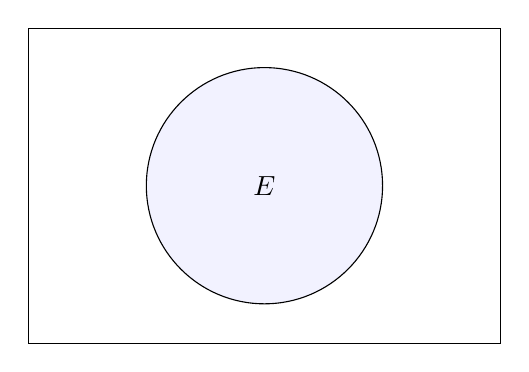
\begin{tikzpicture}
\draw (0,0) rectangle (6,4) node[below left] {$\sS$};
\filldraw[fill=blue!5] (3,2) circle (1.5) node {$E$};
\end{tikzpicture}
\caption{Single event $E$} \label{fig:Single event}
\end{figure}
Now, assuming the area of $E$ is half the area of \sS, we have that the probability of $E$ is the probability that a randomly chosen point on the area of \sS~will be within $E$.

Consider now we let $G = \{\, 4,5,6 \,\}$ be the event that that the number selected is greater than or equal to 4. We have
\par\smallskip
\begin{figure}[h]
\centering
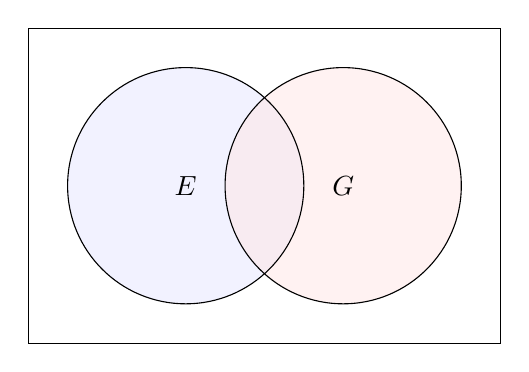
\begin{tikzpicture}

\def\eventE{(2,2) circle (1.5)}
\def\eventG{(4,2) circle (1.5)}

\draw (0,0) rectangle (6,4) node[below left] {$\sS$};

\begin{scope}[fill opacity=0.5]
\fill[blue!10] \eventE;
\fill[red!10] \eventG;
\end{scope}

\draw \eventE node {$E$};
\draw \eventG node {$G$};

\end{tikzpicture}
\caption{Events $E$ and $G$} \label{fig:Events E and G}
\end{figure}
The total shaded region of the Venn diagram, $E \union G$, contains all the sample points of $E$ and $G$. It is the event that any outcome in either $E$ or~$G$, or both, occurs. Thus, $E \union G$ is the event that $E$, $G$ or~both, occurs. Similarly, the union of three events is the event that at least one of the three events occur.

Consider now the intersection $E \intersect G$. It is the set of all the points that are in both $E$ and~$G$, $\{\, 4,6 \,\}$. Thus, it is the event that an outcome in both $E$ and $G$ occurs. So $E \intersect G$ is the event that $E$ and~$G$ both occur. 
\begin{info}
The sets $A \intersect B$ and similarly $A \intersect B \intersect C$ are often denoted as $AB$ and $ABC$ respectively.
\end{info}
Finally, the unshaded space in Figure 4.1 is the set of all outcomes that are not in~$E$. It is the complement of $E$ and is denoted by $\comp{E}$. It is the event that $E$ does not occur.
\begin{info}
Note that the complement of \sS~is the null set, that is $\comp{\sS} = \nullset$, and has a probability of 0.
\end{info}
% ------------------------------------------------- %
\section{De Morgan's Laws}
\begin{theorem}
The following are De Morgan's Laws:
\begin{enumerate}
    \item $\comp{A \union B} = \comp{A} \intersect \comp{B}$
    \item $\comp{A \intersect B} = \comp{A} \union \comp{B}$
\end{enumerate}
\end{theorem}
% Include a proof here #;target
\section{Rules for Unions of Events}
Recall Figure 4.2, copied below.
\par
\begin{figure}[h]
\centering
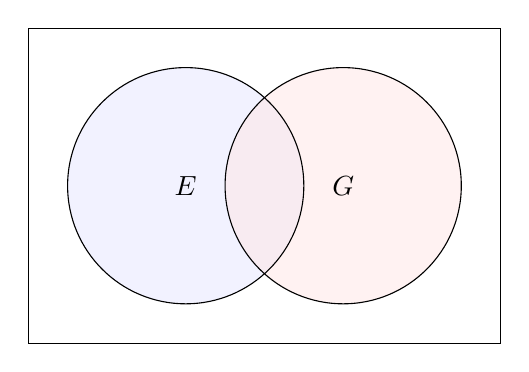
\begin{tikzpicture}

\def\eventE{(2,2) circle (1.5)}
\def\eventG{(4,2) circle (1.5)}

\draw (0,0) rectangle (6,4) node[below left] {$\sS$};

\begin{scope}[fill opacity=0.5]
\fill[blue!10] \eventE;
\fill[red!10] \eventG;
\end{scope}

\draw \eventE node {$E$};
\draw \eventG node {$G$};

\end{tikzpicture}
\repeatcaption{fig:Events E and G}{Events E and G}
\end{figure}
We can see that the area of $E \union G$ is not simply the sum of the areas of $E$ and~$G$. So we have that the probability of $E \union G$ is not simply the sum of the probability of $E$ and $G$. Rather, we must sum the probabilities and subtract the intersection (which gets included twice in the sum) to obtain $P(E \union G)$.
\begin{theorem}
For any events, $A$ and $B$, in a sample space, we have
\[
    P(A \union B) = P(A) + P(B) - P(A \intersect B)
\]
\end{theorem}
\begin{example}
A number between 1 and 6 inclusive is chosen randomly. Let $E = \{\, 2,4,6 \,\}$ be the event the number is odd and let $G = \{\, 4,5,6 \,\}$ be the event that the number is greater than or equal to 4.
\par\smallskip
The probability of the number being even \textbf{or} greater than 4 is $P(E \union G)$. Since both $E$ and~$G$ contain 3~points of the six in the sample space, $P(E) = P(G) = 1/2$. Thus, we can see clearly that $P(E \union G) \neq P(E) + P(G) = 1$ since $\{\, 1 \,\}$ is not in $E$ or $G$ and has a probability of 1/6. Now, note $E \intersect G = \{\, 4,6 \,\}$, so $P(E \intersect G) = 1/3$. We have
\[
    P(E \union G) = P(E) + P(G) - P(E \intersect G) = 1/2 + 1/2 - 1/3 = 2/3
\]
\end{example}
\pagebreak[3]
Now consider the case of the union of three events.\par
\begin{figure}[ht]
\centering
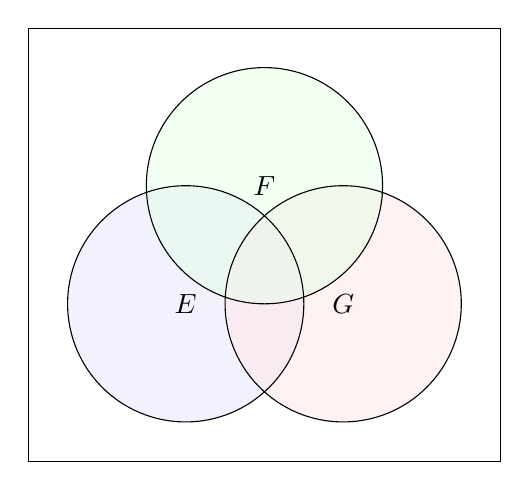
\begin{tikzpicture}

\def\eventE{(2,2) circle (1.5)}
\def\eventG{(4,2) circle (1.5)}
\def\eventF{(3,3.5) circle (1.5)}

\draw (0,0) rectangle (6,5.5) node[below left] {$\sS$};

\begin{scope}[fill opacity=0.5]
\fill[blue!10] \eventE;
\fill[red!10] \eventG;
\fill[green!10] \eventF;
\end{scope}

\draw \eventE node {$E$};
\draw \eventG node {$G$};
\draw \eventF node {$F$};

\end{tikzpicture}
\caption{Three events} \label{fig:Three events}
\end{figure}
Let $A_I$ be the area on the Venn diagram of the event $I$. The area of the union once again is not simply the sum of the areas ($A_E + A_G + A_F$). Instead we can reason out that when we add the three areas we include $A_{E \intersect G}$, $A_{G \intersect F}$, and $A_{F \intersect E}$ twice each and $A_{E \intersect G \intersect F}$ three times. The sum of these doubly counted areas ($A_{E \intersect G} + A_{G \intersect F} + A_{F \intersect E}$) also includes $A_{E \intersect G \intersect F}$ three times. Thus, when we subtract the area of the doubly counted segments, $A_{E \intersect G \intersect F}$ is also subtracted three times leaving this area unaccounted for. Therefore we then add $A_{E \intersect G \intersect F}$ to find the complete area of $E \union G \union F$.
\begin{theorem}
For any events, $A$, $B$ and $C$, in a sample space, we have
\[
    P(A \union B \union C) = P(A) + P(B) + P(C) - P(A \intersect B) - P(B \intersect C) - P(C \intersect A) + P(A \intersect B \intersect C)
\]
\end{theorem}
\section{Mutually Exclusive Events}
Events $A$ and $B$ are mutually exclusive if and only if $A \intersect B = \nullset$. More simply, the events $A$ and $B$ cannot both occur in one experiment because they share no points in common and only one sample point is achieved.
\par\smallskip
In general, events $A_1,A_2,A_3,\ldots,A_n$ are mutually exclusive if and only if $A_i \intersect A_j = \nullset \for\all i \neq j$. This means that at most one of these events may occur in any one experiment.
\subsection*{Probability of the Unions of Mutually Exclusive Events}
Consider the Venn diagram of two mutually exclusive events, $E$ and $G$.
\begin{figure}[htp]
\centering
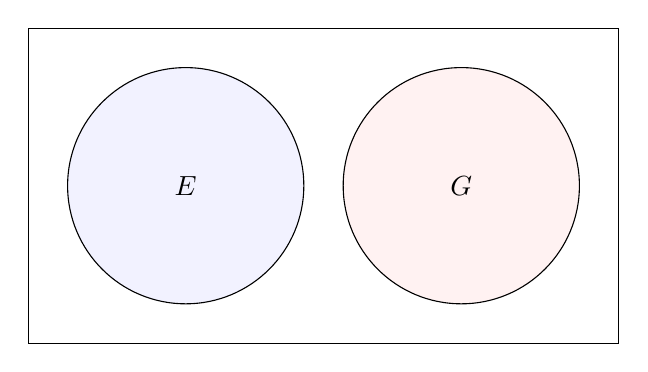
\begin{tikzpicture}

\def\eventE{(2,2) circle (1.5)}
\def\eventG{(5.5,2) circle (1.5)}

\draw (0,0) rectangle (7.5,4) node[below left] {$\sS$};

\begin{scope}[fill opacity=0.5]
\fill[blue!10] \eventE;
\fill[red!10] \eventG;
\end{scope}

\draw \eventE node {$E$};
\draw \eventG node {$G$};

\end{tikzpicture}
\caption{Two mutually exclusive events} \label{fig:Two mutually exclusive events}
\end{figure}
Clearly the probability of the intersection of two mutually exclusive events is 0, since it doesn't contains any sample points. So we have 
\[
    P(E \intersect G) = 0    
\]
Another intrinsic property of mutually exclusive events that we can see on a Venn diagram is that the area of $E \union G$ is the sum of the areas of $E$ and $G$. Therefore, unlike in previous examples, the probability of $E \union G$ is the sum of the probabilities of $E$ and $G$.
\begin{theorem}
For mutually exclusve events, $A$ and $B$, in a sample space, we have
\[
    P(A \union B) = P(A) + P(B)
\]
\end{theorem}
\begin{theorem}
More generally for $n$ mutually exclusive events, $A_1,A_2,\ldots,A_n$, in a sample space, we have
\[
    P(A_1 \union A_2 \union \cdots \union A_n) = P(A_1) + P(A_2) + \cdots + P(A_n) = \sum_{i = 1}^{n} P(A_i)
\]
\end{theorem}
\subsection*{Probabilities of Complements}
\begin{theorem}
For any event $A$, we have
\[
    P(A) = 1 - P(\comp{A})
\]
\end{theorem}
\begin{proof}
Recall the complement of an event consists of all the sample points not in the event. Thus, for any event~$A$, its complement~$\comp{A}$ contains no points in common with~$A$. So $A \intersect \comp{A} = \nullset$ and $A$ and~$\comp{A}$ are mutually exclusive, by~definition. Now, consider $A \union \comp{A}$, it spans the whole of the sample space so we have $P(A \union \comp{A}) = 1$ and since $A$ and $\comp{A}$ are mutually exclusive, we have
\[
    P(A) + P(\comp{A}) = 1
\]
and it follows that $P(A) = 1 - P(\comp{A})$, as required.
\end{proof}
\section{Independence of Events}
Events $A$ and $B$ are said to be independent if and only if $P(A \intersect B) = P(A)P(B)$. Otherwise they are dependent events.
\par\smallskip
In general, events $A_1,A_2,A_3\ldots,A_n$ are independent if and only if 
\[
    P(A_{i_1} \intersect A_{i_2} \intersect A_{i_3} \intersect \cdots \intersect A_{i_n}) = P(A_{i_1}) + P(A_{i_2}) + P(A_{i_3}) + \cdots + P(A_{i_n})
\]
for all sets $\{\, i_1,i_2,i_3,\ldots,i_k \,\}$ of distinct subscripts chosen from $\{\, 1,2,3,\ldots,n \,\}$.
\begin{example}
Consider an experiment in which a fair die is tossed twice. We define the following events:
\begin{itemize}[noitemsep, topsep=4pt plus 2pt minus 1pt]
    \item $A$: The first number rolled is a six
    \item $B$: The second number rolled is a six
    \item $C$: The sum of the numbers rolled is less than or equal to seven
    \item $D$: The sum of the numbers rolled is equal to seven
\end{itemize}
Suppose the event $A$ occurs. Does this have any impact on the probability of $B, C$ or $D$ occurring?
\par\smallskip
It is quite clear to see that the events $A$ and $B$ are independent events since rolling a six on the first toss has no impact on the number that will be rolled on the second toss. Now, events $B$ and $C$ from the onset appear to be dependent since if you roll a six on the first toss you must roll a one to make your total less than or equal to seven. To confirm this consider the sample space
\[
    \left\{
        \begin{array}{c@{,\ }c@{,\ }c@{,\ }c@{,\ }c@{,\ }c}
            (1,1) & (1,2) & (1,3) & (1,4) & (1,5) & (1,6) \\
            (2,1) & (2,2) & (2,3) & (2,4) & (2,5) & (2,6) \\
            (3,1) & (3,2) & (3,3) & (3,4) & (3,5) & (3,6) \\
            (4,1) & (4,2) & (4,3) & (4,4) & (4,5) & (4,6) \\
            (5,1) & (5,2) & (5,3) & (5,4) & (5,5) & (5,6) \\
            (6,1) & (6,2) & (6,3) & (6,4) & (6,5) & (6,6) \\
        \end{array}
    \right\}
\]
We can count that 21 of the sample points have sums less than or equal to seven. So the probability of $C$ occurring is $P(C) = 21/36 = 7/12$. We also have that $P(A) = 1/6$. So $P(A)P(C) = 7/72$ but we can count that $A \intersect C$ contains only one sample point and hence has a probability of $1/36$. Thus, $P(A)P(C) \neq P(A \intersect C)$ so $A$ and $C$ are dependent events.
\par\smallskip
At first glance, we see that upon rolling a six as the first number you must roll a 1 for the sum to equal seven. So at first glance, events $A$ and $D$ seem to be independent however it would be na\"\i ve to assume this. We can count from the sample space that event $D$ contains 6 points and so has a probability~$P(D) = 6/36 = 1/6$ and $P(A) = 1/6$. So $P(A)P(D) = 1/36$. Now, we can count that the event $A \intersect D$ contains only one point, (1,6) and so has a probability~$P(A \intersect D) = 1/36$. Therefore, $P(A \intersect D) = P(A)P(D)$ and the events $A$ and~$D$ are independent.
\end{example}
\section{Conditional Probability}
Often we need to calculate the probability of some event~$A$ occurring while knowing that some other event~$B$ has already occurred. We call this the conditional probability of $A$ \textbf{given} $B$ and denote it by $P(A \given B)$.
\par\smallskip
The conditional probability of event~$A$, given event~$B$, is
\[
    P(A \given B) = \frac{P(A \intersect B)}{P(B)}\for P(B) > 0
\]
\begin{theorem}
For any two events~$A$ and~$B$ defined on the same sample space, with $P(A) > 0$ and $P(B) > 0$, events~$A$ and~$B$ are independent if and only if $P(A \given B) = P(A)$ or $P(B \given A) = P(B)$.
\end{theorem}
\begin{proof}
\begin{align*}
    P(A \given B) &= \frac{P(A \intersect B)}{P(B)} \\
    \ifo 
    P(A \intersect B) &= P(A \given B)P(B)
\end{align*}
and by definition of independence,~$A$ and~$B$ are independent if and only if $P(A \intersect B) = P(A)P(B)$ which is true if and only if $P(A \given B) = P(A)$. Without loss of generality we can swap events~$A$ and~$B$ and arrive at the conclusion.
\end{proof}
\subsection*{Product Rules}
\begin{theorem}
Let $A, B, C$ and~$D$ be events on a sample space, with $P(A), P(B), P(C), P(D) > 0$. We have
\begin{align*}
    P(A \intersect B) &= P(A)P(B \given A) \\
    P(A \intersect B \intersect C) &= P(A)P(B \given A)P(C \given A \intersect B) \\
    P(A \intersect B \intersect C \intersect D) &=
    P(A)P(B \given A)P(C \given A \intersect B)P(D \given A \intersect B \intersect C) \\
\end{align*}
and so on$\ldots$
\end{theorem}
\subsection*{Law of Total Probability}
\begin{theorem}
Let $A_1, A_2, A_3,\ldots,A_k$ be mutually exclusive events on a sample space and let $B$ be an event on the same sample space. We have
\[
    P(B) = P(B \intersect A_1) + P(B \intersect A_2) + P(B \intersect A_3) + \cdots + P(B \intersect A_k)
    = \sum_{i = 1}^{k} P(A_i)P(B \given A_i)
\]
\end{theorem}
\subsection*{Bayes' Theorem}
\begin{theorem}
Let $A$ and~$B$ be events on a sample space, with $P(B) > 0$. We have
\[
    P(A \given B) = \frac{P(B \given A)P(A)}{P(B)}
    = \frac{P(B \given A)P(A)}{P(B \given \comp{A})P(\comp{A}) + P(B \given A)P(A)}
\]
\end{theorem}
\begin{proof}
\begin{align*}
    P(A \given B)
    &= \frac{P(A \intersect B)}{P(B)} 
    = \frac{P(B \given A)P(A)}{P(B)}\by{Theorem 4.7.2 (Product Rule)} \\
    &= \frac{P(B \given A)P(A)}{P(A \intersect B) + P(\comp{A} \intersect B)}
    \by{Theorem 4.7.3 (Law of Total Probability)} \\
    &= \frac{P(B \given A)P(A)}{P(B \given \comp{A})P(\comp{A}) + P(B \given A)P(A)}\by{Theorem 4.7.2 (Product Rule)}
\end{align*}
\end{proof}
\begin{info}
Bayes' Theorem allows us to find the conditional probability of some event~$A$ given~$B$, in terms of the probability of~$B$ given~$A$. It allows us calculate conditional probabilities using the reversed order of conditioning.
\end{info}

\chapter{Conditional Probability}
Often we need to calculate the probability of some event~$A$ occurring while knowing that some other event~$B$ has already occurred. We call this the conditional probability of $A$ \textbf{given} $B$ and denote it by $P(A \given B)$.
\par\smallskip
The conditional probability of event~$A$, given event~$B$, is
\[
    P(A \given B) = \frac{P(A \intersect B)}{P(B)}\for P(B) > 0
\]
\section{Theorems and Rules for Conditional Probability}
\begin{theorem}
For any two events~$A$ and~$B$ defined on the same sample space, with $P(A) > 0$ and $P(B) > 0$, events~$A$ and~$B$ are independent if and only if $P(A \given B) = P(A)$ or $P(B \given A) = P(B)$.
\end{theorem}
\begin{proof}
\begin{align*}
    P(A \given B) &= \frac{P(A \intersect B)}{P(B)} \\
    \ifo 
    P(A \intersect B) &= P(A \given B)P(B)
\end{align*}
and by definition of independence,~$A$ and~$B$ are independent if and only if $P(A \intersect B) = P(A)P(B)$ which is true if and only if $P(A \given B) = P(A)$. Without loss of generality we can swap events~$A$ and~$B$ and arrive at the conclusion.
\end{proof}
\subsection*{Product Rules}
\begin{theorem}
Let $A, B, C$ and~$D$ be events on a sample space, with $P(A), P(B), P(C), P(D) > 0$. We have
\begin{align*}
    P(A \intersect B) &= P(A)P(B \given A) \\
    P(A \intersect B \intersect C) &= P(A)P(B \given A)P(C \given A \intersect B) \\
    P(A \intersect B \intersect C \intersect D) &=
    P(A)P(B \given A)P(C \given A \intersect B)P(D \given A \intersect B \intersect C) \\
\end{align*}
and so on$\ldots$
\end{theorem}
\begin{proof}
The first statement come directly from the definition of conditional probability
\[
    P(A)P(B \given A) = P(A) \frac{P(A \intersect B)}{P(A)} = P(A \intersect B)
\]
For the second we have
\begin{align*}
    P(A)P(B \given A)P(C \given A \intersect B)
    &= P(A \intersect B)P(C \given A \intersect B)
    &\by{the first statement} \\
    &= P(A \intersect B) \frac{P(A \intersect B \intersect C)}{P(A \intersect B)}
    &\by{definition of conditional probability} \\
    &= P(A \intersect B \intersect C)
\end{align*}
and so on$\ldots$
\end{proof}
\subsection*{Law of Total Probability}
\begin{theorem}
Let $A_1, A_2, A_3,\ldots,A_k$ be mutually exclusive events on a sample space and let $B$ be an event on the same sample space. We have
\[
    P(B) = P(B \intersect A_1) + P(B \intersect A_2) + P(B \intersect A_3) + \cdots + P(B \intersect A_k)
    = \sum_{i = 1}^{k} P(A_i)P(B \given A_i)
\]
\end{theorem}
\begin{proof}
Note that the events $A_i \intersect B$ for $1 \leq i \leq k$ are all mutually exclusive events since $A_i$'s are mutually exclusive. Thus, the union of the $A_i \intersect B$'s is $B$, that is 
\[
    (A_1 \intersect B) \union (A_2 \intersect B) \union (A_3 \intersect B) \union \cdots \union (A_k \intersect B) = B
\]
So by Theorem 4.5.1, we have
\[
    P(B) = P(A_1 \intersect B) + P(A_2 \intersect B) + P(A_3 \intersect B) + \cdots + P(A_k \intersect B)
\]
and by Theorem 5.1.2 (Product Rule), we have
\[
    P(B) = P(A_1)P(B \given A_1) + P(A_2)P(B \given A_2) + P(A_3)P(B \given A_3) + \cdots + P(A_k)P(B \given A_k) = \sum_{i = 1}^{k} P(A_i)P(B \given A_i)
\]
as required.
\end{proof}
\subsection*{Bayes' Theorem}
\begin{theorem}
Let $A$ and~$B$ be events on a sample space, with $P(B) > 0$. We have
\[
    P(A \given B) = \frac{P(B \given A)P(A)}{P(B)}
    = \frac{P(B \given A)P(A)}{P(B \given \comp{A})P(\comp{A}) + P(B \given A)P(A)}
\]
\end{theorem}
\begin{proof}
\begin{align*}
    P(A \given B)
    &= \frac{P(A \intersect B)}{P(B)} 
    = \frac{P(B \given A)P(A)}{P(B)}\by{Theorem 4.7.2 (Product Rule)} \\
    &= \frac{P(B \given A)P(A)}{P(A \intersect B) + P(\comp{A} \intersect B)}
    \by{Theorem 4.7.3 (Law of Total Probability)} \\
    &= \frac{P(B \given A)P(A)}{P(B \given \comp{A})P(\comp{A}) + P(B \given A)P(A)}\by{Theorem 4.7.2 (Product Rule)}
\end{align*}
\end{proof}
\begin{info}
Bayes' Theorem allows us to find the conditional probability of some event~$A$ given~$B$, in terms of the probability of~$B$ given~$A$. It allows us calculate conditional probabilities using the reversed order of conditioning.
\end{info}
\section{Tree Diagrams}
Tree diagrams are a technique that we can use to keep track of conditional probabilities. We start from a single node and draw new branches to separate nodes for each event. Each node represents the event occurring. On each branch we write the probability of event it leads to occurring. To find the probability of any node we multiply the probabilities of the branches leading to the node.
\begin{figure}[htp]
\centering
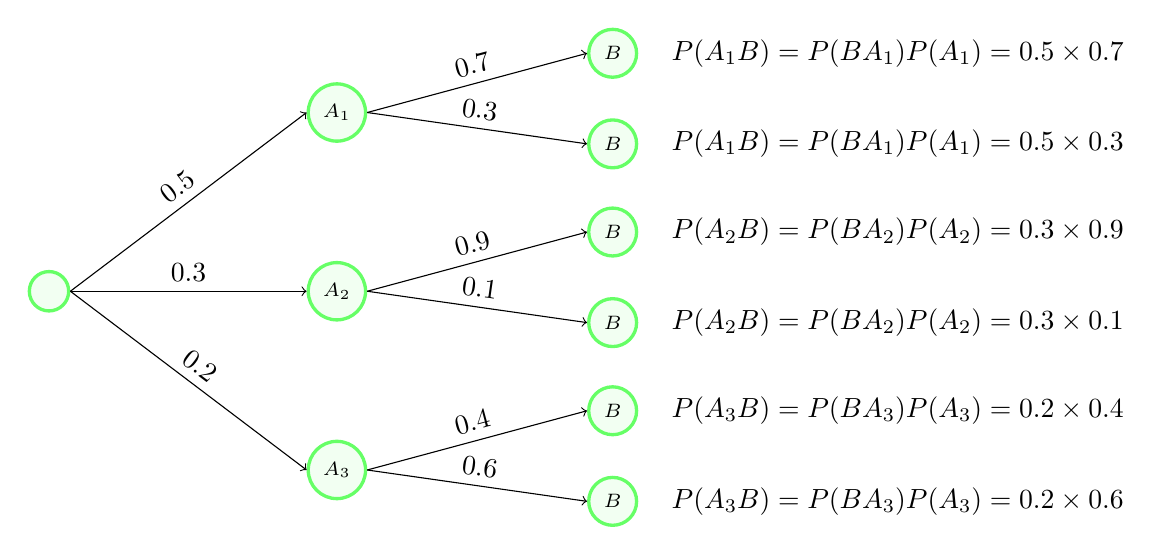
\begin{tikzpicture}[
roundnode/.style={circle, draw=green!60, fill=green!5, very thick, minimum size=5mm},
]
%Nodes
\node[roundnode]        (root)                              {};
\node[roundnode]        (A2)        [right=3cm of root]                 {$\scriptstyle A_2$};
\node[roundnode]        (A1)        [above=1.5cm of A2]                 {$\scriptstyle A_1$};
\node[roundnode]        (A3)        [below=1.5cm of A2]                 {$\scriptstyle A_3$};
\node[roundnode]        (A1B)       [above right=0.25cm and 3cm of A1]   {$\scriptstyle B$};
\node[roundnode]        (A1compB)   [below=0.5cm of A1B]                {$\scriptstyle\comp{B}$};
\node[roundnode]        (A2B)       [above right=0.25cm and 3cm of A2]   {$\scriptstyle B$};
\node[roundnode]        (A2compB)   [below=0.5cm of A2B]                {$\scriptstyle\comp{B}$};
\node[roundnode]        (A3B)       [above right=0.25cm and 3cm of A3]   {$\scriptstyle B$};
\node[roundnode]        (A3compB)   [below=0.5cm of A3B]                {$\scriptstyle\comp{B}$};
 
%Lines
\draw[->] (root.east) -- (A1.west) node[midway, sloped, above] {0.5};
\draw[->] (root.east) -- (A2.west) node[midway, sloped, above] {0.3};
\draw[->] (root.east) -- (A3.west) node[midway, sloped, above] {0.2};
\draw[->] (A1.east) -- (A1B.west) node[midway, sloped, above] {0.7};
\draw[->] (A1.east) -- (A1compB.west) node[midway, sloped, above] {0.3};
\draw[->] (A2.east) -- (A2B.west) node[midway, sloped, above] {0.9};
\draw[->] (A2.east) -- (A2compB.west) node[midway, sloped, above] {0.1};
\draw[->] (A3.east) -- (A3B.west) node[midway, sloped, above] {0.4};
\draw[->] (A3.east) -- (A3compB.west) node[midway, sloped, above] {0.6};

%Probabilities
\node [right=3mm of A1B]
    {$P(A_1 \intersect B) = P(B \given A_1)P(A_1) = 0.5 \times 0.7$};
\node [right=3mm of A1compB]
    {$P(A_1 \intersect \comp{B}) = P(\comp{B} \given A_1)P(A_1) = 0.5 \times 0.3$};
\node [right=3mm of A2B]
    {$P(A_2 \intersect B) = P(B \given A_2)P(A_2) = 0.3 \times 0.9$};
\node [right=3mm of A2compB]
    {$P(A_2 \intersect \comp{B}) = P(\comp{B} \given A_2)P(A_2) = 0.3 \times 0.1$};
\node [right=3mm of A3B]
    {$P(A_3 \intersect B) = P(B \given A_3)P(A_3) = 0.2 \times 0.4$};
\node [right=3mm of A3compB]
    {$P(A_3 \intersect \comp{B}) = P(\comp{B} \given A_3)P(A_3) = 0.2 \times 0.6$};
\end{tikzpicture}
\caption{Tree diagram} \label{fig:Tree diagram}
\end{figure}
\begin{info}
The probability of all the the branches leading outward from each node must sum to~ 1 since at least one outcome must occur.
\end{info}
\chapter{Useful Sums and Series}
This chapter includes a few useful sums and series that show up in the following chapters.
\section{Geometric Series}
\[
    \sum_{i = 0}^{n-1} r^i = 1 + r + r^2 + \cdots + r^{n-1} = \frac{1-r^n}{1-r}
\]
For $\abs{r} < 1$, we have
\[
    \sum_{i = 0}^{\infty} r^i = 1 + r + r^2 + \cdots = \frac{1}{1-r}
\]
\begin{info}
Other identities can be obtained from this one by differentiation. For example we have
\[
    \deriv r\sum_{i = 0}^{\infty} r^i = \sum_{i = 0}^{\infty} ir^{i-1} = \deriv r\,\frac{1}{1-r} = \frac{1}{(1-r)^2}
\]
\end{info}
\section{Binomial Theorem}
The binomial theorem describes the algebraic expansion of powers of a polynomial.
\[
    (1 + t)^n = 1 + \binom{n}{1}t^1 + \binom{n}{2}t^2 + \cdots + \binom{n}{n}t^n = \sum_{x = 0}^{n} \binom{n}{x} t^x
\]
for any positive integer $n$ and real number $t$.
\par\smallskip
A more general form of this theorem that holds even when $n$ is not a positive~integer is
\[
    (1 + t)^n = \sum_{x = 0}^{\infty} \binom{n}{x} t^x,\:\for \abs{t} < 1
\]
\begin{info}
It is an important skill to be able to recognize if an infinite, or otherwise, polynomial with binomial coefficients can be reduced to a simple polynomial raised to a power.
\end{info}
\section{Multinomial Theorem}
The multinomial theorem is a generalization of the binomial theorem. It describes the algebraic expansion of powers of a sum in terms of powers of the terms in the sum.
\[
    (x_1 + x_2 + \cdots + x_m)^n = \sum_{k_1 + k_2 + \cdots + k_m = n} \binom{n}{k_1,k_2,\ldots,k_m} \prod_{t = 1}^{m} x_t^{k_t}
\]
Another common form in which this theorem may be represented is
\[
    (x_1 + x_2 + \cdots + x_m)^n 
    = \sum_{k_1 + k_2 + \cdots + k_m = n} \frac{1}{k_1!\,k_2!\cdots k_m!}(x_1^{k_1}x_2^{k_2}\cdots x_m^{k_m})
\]
\begin{info}
The summation is over all non-negative integers, $k_1,k_2,\ldots,k_m$ such that $k_1 + k_2 + \cdots + k_m = n$
\end{info}
\section{Hypergeometric Identitiy}
\[
    \sum_{x = 0}^{\infty} \binom{a}{x} \binom{b}{n-x} = \binom{a + b}{n}
\]
\begin{proof}
We begin with the equality
\[
    (1 + y)^{a + b} = (1 + y)^a \times (1 + y)^b
\]
Now by Binomial Theorem we have
\[
    \sum_{k = 0}^{a + b} \binom{a + b}{k} y^k = \sum_{i = 0}^{a} \binom{a}{i} y^i \times \sum_{j = 0}^{b} \binom{b}{j} y^j
\]
Consider the coefficient of $y^k$ on the right hand side. It is the sum of all the binomial terms such that $i + j = k$. Thus, the coefficient of $y^k$ on the right hand side is
\[
    \sum_{i = 0}^{\min\{\, a,k \,\}} \binom{a}{i} \binom{b}{k-i}
\]
and since when $i > a$ or $i > k$ the term is 0 we can increase the sum to infinity. Thus, since the coefficient on the right hand side is equal to that on the left hand side we have
\[
    \binom{a + b}{k} = \sum_{i = 0}^{\infty} \binom{a}{i} \binom{b}{k-i}
\]
\end{proof}
\begin{info}
When $x$ becomes significantly large, the terms of the summation become 0 since 
\[
    \binom{n}{x} = \binom{n}{n-x} = 0,\:\for x > n
\]
\end{info}

\chapter{Discrete Random Variables and Probability Functions}
\section{Random Variables}
A random variable (\rv~for short) is a numerical valued variable that represents the outcome of an experiment or process. Every random variable has a range associated with it, which is the set of all possible values the \rv~can take. We denote random variables by capital letters, e.g., $A$, $X$, $Z$.
\begin{example}
Suppose an experiment consists of tossing a coin three times. Let the random variable $X$ be the number of heads that are rolled. And let the random variable $Y$ be the number of tails rolled. Now, we have a nice short hand in that $X = 2$ is equivalent to the statement ``two heads were rolled''.
\par\smallskip
Moreover, we have useful equalities such as $X + Y = 3$ and $X = 3 - Y$. 

The ranges of $X$ and $Y$ are both $\{\, 0,1,2,3 \,\}$.
\end{example}
\begin{info}
It is very important to understand the purpose of \rv's since the remainder of this course features them heavily.
\end{info}
The formal definition of a random variable is a function that assigns a real number to each point in a sample space.
\begin{example}
Consider the same experiment as above. The sample space is
\[
    \{\, \text{HHH, HHT, HTH, HTT, THH, THT, TTH, TTT} \,\}
\]
Let us define $X$ the number of heads that are rolled and the sample point $a = \text{HHT}$. The value of the function $X(a) = 2$ it is found by counting the number of heads in $a$. The range of $X$ is $\{\, 0,1,2,3 \,\}$. Each of the outcomes $X=x$ represents an event, simple or compound. In this case they are:
\begin{center}
\begin{tabular}{c|r}
    $X$     & Event \\
    \hline
    0       & $\{\, \text{TTT} \,\}$ \\
    1       & $\{\, \text{TTH, THT, HTT} \,\}$ \\
    2       & $\{\, \text{THH, HTH, HHT} \,\}$ \\
    3       & $\{\, \text{HHH} \,\}$ \\
\end{tabular}
\end{center}
\end{example}
Since some outcome in the range must always occur for a random variable for each event in the sample space, the events of a random variable are mutually exclusive subsets of the sample space such that their union is the total sample space. For \rv~$X$ and outcome $x$, we have $X = x$ represents some event and we are interested in calculating its probability. We denote the probability of $X = x$ by $P(X = x)$.
\begin{info}
Since the union of the events of values of a random variable is the total sample space, we have
\[
    \sum_{x \in \range{X}} P(X=x) = 1
\]
\end{info}
\subsection*{Discrete Random Variables}
Discrete random variables take integer values or, more generally, values in a countable set. Recall that a set is countable if its elements can be placed in a one-to-one correspondence with a subset of the positive integers.
\subsection*{Continuous Random Variables}
Continuous random variables (which are not the focus of this chapter) take values in some interval of real numbers like $(0,1)$ or $(0,\infty)$ or $(\infty,\infty)$. You should be aware that there are infinitely numerical non-integer values that a \rv~with $\range{0,1}$ could take. The values are separated by infinitesimally small intervals.
\section{Probability Function}
The probability function of a discrete random variable $X$ is a function that maps the value of $X$ to the probability of that value. The probability function is represented by 
\[
    f(x) = P(X = x)\for x\in\range{X}
\]
The set of pairs $\{\, (x,f(x)) \ssep x\in\range{X} \,\}$ is called the \textbf{probability distribution} of~$X$.

\subsection*{Properties of Probability Functions}
The following two properties hold for all probability functions (on discrete \rv's).
\begin{itemize}
    \item $f(x) \geq 0 \for\all x\in\range{X}$
    \item $\sum\limits_{x\in\range{X}} f(x) = 1$
\end{itemize}
\section{Cumulative Distribution Function}
Another common function used to describe a probability model is the cumulative distribution function, usually denoted by $F(x)$. It is defined to be
\[
    F(x) = P(X \leq x) \for\all x\in\range{X}
\]
Not that because the events ``$X = x$'' and ``$X = y$'' for $x \neq y$ are mutually exclusive we have
\[
    F(x) = P(X \leq x) = \sum_{z = 0}^{x} P(X = z)  \for\all x\in\range{X}
\]
It is the sum of the probabilities that the random variable takes values less than or equal to $x$.
\subsection*{Properties of Cumulative Distribution Functions}
The following four properties hold for all cumulative distribution functions.
\begin{itemize}
    \item $F(x)$ is a non-decreasing function
    \item $0 \leq F(x) \leq 1 \for\all x\in\sR$
    \item $\lim\limits_{x \tendsto -\infty} F(x) = 0$
    \item $\lim\limits_{x \tendsto \infty} F(x) = 1$
\end{itemize}
\chapter{Discrete Distributions}
As we briefly mentioned in the previous chapter, \textbf{probability distributions} are the set of pairs~$(x,f(x))$ for all possible outcomes~$x$ of a random variable~$X$. Many probability distributions appear commonly on \rv's of similar ``real-life'' processes. In this chapter we define a few of these common distributions on discrete random variables, when they occur and how to use them to calculate probabilities.
\begin{info}
It is important to understand distributions early-on. Distributions, probability functions and cumulative distribution functions are defined on random variables \textbf{not} experiments/processes or sample spaces.
\end{info}

\section{Uniform Distribution}
Suppose $X$ can take a finite set of consecutive values with each of the values being equally likely. That is $\range{X} = \{\, a,a+1,a+2,\ldots,b \,\}$ with each of $a,a+1,a+2,\ldots,b$ being equally likely. Then $X$ has a discrete uniform distribution and we denote it \\
$X \dist \duni$
\[
    f(x) = P(X = x) = \left\{
    \begin{array}{c@{\hspace{1em}}l}
        \displaystyle\frac{1}{b - a + 1} & \for\all x\in\range{X} \\[1em]
         0 & \ow 
    \end{array}\right.
\]
\begin{theory}{Derivation of Probability Function}
The probability of each value of the \rv~is easy to calculate since they are all equal and must add up to 1. Therefore, $k \times P(X = a) = 1$ where $k$ is the number of possible values of $X$. The number of possible values of $X$ is $b - (a - 1) = b - a + 1$ since $\range{X}$ is between $a$ and $b$ inclusive.
\end{theory}
\begin{info}
Another way to define the probability of each value of a random variable with this sample space is 
\[
\frac{1}{\text{Number of possible values in $\range{X}$}}
\]
\end{info}
\section{Hypergeometric Distribution}
Suppose we have a collections of $N$ objects which can be classified into two different types, successes and failures. There are $r$ successes and $N -r$ failures. We pick $n$ objects at random without replacement, and let the random variable $X$ be the number of successes obtained. $X$ has a hypergeometric distribution and we denote it \\
$X\dist\hype$
\[
    f(x) = P(X = x) =
    \frac{\displaystyle\binom{r}{x} \binom{N-r}{n-x}}{\displaystyle\binom{N}{n}},\:\for x\leq\min(r,n)
\]
\begin{theory}{Derivation of Probability Function}
We will use the counting techniques we previously learnt to calculate the probability function. We note that there are $\binom{N}{n}$ ways to select $n$ objects from the total of $N$ so the sample space contains $\binom{N}{n}$~points. Now the number of ways of choosing $x$ successes from the total of $r$ is $\binom{r}{x}$ \textbf{and independently} the number of ways to choose the remainder of objects, $n-x$, from the total remaining objects, $N - r$, is $\binom{N - r}{n - x}$. Thus the probability of~$X = x$ by the multiplication rule is the product of those expressions divided by the number of points in the sample space, $\frac{\binom{r}{x}\binom{N-r}{n-x}}{\binom{N}{n}}$.
\end{theory}
\begin{info}
It is important to understand that the terms ``successes'' and ``failures'' are simply placeholder that represent a type of outcome and its complement. They could be replaced by ``wins'' and ``losses'', ``whites'' and ``colors'', or any other titles that are distinct groups with a union that spans the whole sample space.
\end{info}
\begin{info}
    This is used when we know how many items (n) are chosen at random from a set with two different types and we know the amount of each type in the set.
\end{info}
\begin{example}
There is a basket with 11 fruit, 9 apples and 2 oranges. 4 fruit are picked at random from the basket. Let random variable $X$ be the number of apples selected. Find $f(x)=P(X=x)$. Then find $f(3)$. \\
$X\dist\hype$. $N=11,n=4,r=9$.
\[
    f(x) = P(X = x) = \displaystyle\frac{\displaystyle\binom{9}{x} \binom{2}{4-x}} {\displaystyle\binom{11}{4}},\:\for x \leq 4
\]
Hence 
\[
    f(7) = P(X = 7) = \displaystyle\frac{\displaystyle\binom{9}{3} \binom{2}{1}} {\displaystyle\binom{11}{4}} \approx 0.509
\]
\end{example}
\begin{example}
15 cards are drawn from a deck of 52 at random. Let $X$ be the number of red cards drawn. Find $f(x)=P(X=x)$. Then find $f(7)$. \\
$X\dist\hype$. $N=52,n=15,r=26$.
\[
    f(x) = P(X = x) = \displaystyle\frac{\displaystyle\binom{26}{x} \binom{26}{15-x}} {\displaystyle\binom{52}{15}},\:\for x \leq 15
\]
Hence \[
    f(7) = P(X = 7) = \displaystyle\frac{\displaystyle\binom{26}{7} \binom{26}{8}} {\displaystyle\binom{52}{15}} \approx 0.229
\]
\end{example}
\section{Binomial Distribution}
Suppose we have an experiment with two distinct outcomes, success and failure, with the probability of a success being $p$ and a failure being $(1-p)$. The experiment is repeated $n$ times independently (these are called trials). Let the random variable $X$ be the number of successes obtained. $X$ has a binomial distribution. \\
$X\dist\bino(n,p)$
\[
    f(x) = P(X = x) = \displaystyle\binom{n}{x}p^x (1-p)^{n-x},\:\for x=1,\ldots,n
\]
\begin{theory}{Derivation of Probability Function}
Since there are $n$ positions in which to put the $x$ successes there are $\binom{n}{x}$ unique arrangements of successes and failures that satisfy ``$X = x$''. Each of these arrangements has probability $p^x (1-p)^{n-x}$ since the probability of obtaining $x$ successes is $p^x$ and the probability of obtaining $n-x$ failures is $(1-p)^{n-x}$. So the probability that $X = x$, that is that any of the arrangements occur, is the sum of the probability of each unique arrangement, $\binom{n}{x}p^x (1-p)^{n-x}$.
\end{theory}
\begin{info}
The above formula describes the probability of $x$ success and $(n-x)$ failures multiplied by the number of different ways of arranging those successes within the total number of trials of the experiment.
\end{info}
\begin{info}
Each of the n individual experiments is called a ``Bernoulli trial'' and the entire process of n trials is called a Bernoulli process or a Binomial process.
\end{info}
\begin{example}
A loaded coin is flipped 10 times, with a probability of a heads occurring being 0.4. Let random variable $X$ be the number of heads that occur. Find $f(x)=P(X=x)$, then find $f(3)$. \\
$X\dist\bino(10,0.4)$.
\[
    f(x) = P(X = x) = \displaystyle\binom{10}{x} (0.4)^x (0.6)^{10-x},\:\for x = 1,\ldots,10
\]
Hence 
\[
    f(3) = P(X = 3) = \displaystyle\binom{10}{3} (0.4)^3 (0.6)^7 \approx 0.215
\]
\end{example}
\begin{example}
A football season in a university league has 22 games. The probability of each game being abandoned (because of bad weather or other hazards) is 0.02. Let $X$ be the number of games abandoned throughout the whole season. Find $f(x)=P(X=x)$, then find $f(2)$ and $f(10)$. \\
$X\dist\bino(22,0.02)$.
\[
    f(x) = P(X = x) = \displaystyle\binom{22}{x} (0.02)^x (0.98)^{22-x},\:\for x = 1,\ldots,22
\]
Hence 
\[
    f(2) = P(X = 2) = \displaystyle\binom{22}{2} (0.02)^2 (0.98)^20 \approx 0.062
\]
and 
\[
    f(10) = P(X = 10) = \displaystyle\binom{22}{10} (0.02)^{10} (0.98)^{12} \approx \sn{5.196}{-12}
\]
\end{example}
\subsection{Comparison of Binomial and Hypergeometric Distributions}
The Binomial and Hypergeometric distributions are similar in that they both model the distribution of the number of successes in $n$ trials of an experiment. The difference is that the collection of objects in the hypergeometric distribution is selected from without replacement as apposed the Binomial distribution in which successes and failures do not affect the probability of future outcomes (with replacement).
\begin{info}
The Hypergeometric distribution is used when there is a fixed number of objects (successes and~failures) to choose from.
\par\smallskip
The Binomial distribution is used when there is no fixed number of objects to be selected from and instead we know the constant probability of a success for all the trials.
\end{info}
\begin{example}
Consider Lisa owns a car dealership and has only 750~red cars and 1250~blue cars in stock. A rich~Swedish man enters and picks 50~cars randomly to purchase. Let $X$ be the number of red cars the Swede purchases.
\par\smallskip
Since we know the number of successes (750~red cars) and failures (1250~blue cars) as well as the number of trials, we have that $X \dist \geom$ and 
\[
    f(x) = P(X = x) = \frac{\binom{750}{x} \binom{1250}{50-x}}{\binom{2000}{50}}
\]
Now, consider Lisa has run out of all her stock of cars. She goes to a Swedish car manufacturer's factory which is capable of producing any amount of cars. The factory has a 37.5\% chance of producing a red~car and otherwise produces a blue~car. Lisa orders 50~cars. Let $X$ be the number of red~cars she receives.
\par\smallskip
Since there is no fixed number of cars to choose from but we do know the probability of each car being a success, we have that $X \dist \bino(50, 0.375)$ and
\[
    f(x) = P(X = x) = \binom{50}{x} (0.375)^{x} (0.625)^{50-x}
\]
\end{example}
\subsection{Binomial Estimate of the Hypergeometric Distribution}
When the number of objects to choose from, $N$, is very large and the number of objects being chosen, $n$, is relatively small in a hypergeometric distribution, we have that the probability of a success changes only very slightly due to lack of replacement. Since the number of objects is so large choosing a small number of objects without replacement barely changes the probability of a success so $p$ is relatively constant. Thus we can fairly accurately estimate the distribution with a binomial distribution with the original probability of a success for the first choice.
\begin{example}
Consider the previous example, suppose the rich Swedish man purchased 50 cars from Lisa. What is the probability that he purchases 20 red cars?
\par\smallskip
The number of cars Lisa has in stock is very large and the number of cars being bought is fairly small. Thus we can approximate the distribution with the probability of a success being $750/2000 = 0.375$. We have
\[
    f(20) = P(X = 20) = \binom{50}{20} (0.375)^{20} (0.625)^{30} \approx 0.1072
\]
Now we can calculate the probability using the hypergeometric distribution to determine how good an estimate this is. We have
\[
    f(20) = P(X = 20) = \frac{\binom{750}{20} \binom{1250}{30}}{\binom{2000}{50}} \approx 0.1084
\]
So the approximation is accurate to 2 decimal points.
\end{example}
\section{Negative Binomial Distribution}
This distribution is similar to the binomial distribution. We have an experiment with two distinct outcomes, success and failure, with the probability of a success being~$p$ and a failure being~$(1-p)$. The experiment is repeated until a specified amount of successes, $k$, have been obtained. Let the random variable $X$ be the number of failures obtained before the $k^\text{th}$ success. $X$ has a negative binomial distribution. \\
$X\dist\nbin(k,p)$
\[
    f(x) = P(X = x) = \binom{x+k-1}{x} p^k (1-p)^x,\:\for x = 0,1,2,\ldots
\]
\begin{theory}{Derivation of the Probability Function}
The above formula describes the probability of $x$ failures and $k$ successes multiplied by the number of different ways of arranging those $x$ failures within the total number of candidate trials $n+k-1$. The final trial cannot be a failure as it is the $k$\ts{th} success.
\end{theory}
\begin{info}
The negative binomial distribution is used to model the number of trials of an experiment before the $k$\ts{th}~success. Thus, if we know the number of trials, this distribution is not appropriate.
\end{info}
\begin{example}
A bad driver never stops at red lights and keeps driving and running red lights until he is arrested. The probability of him getting pulled over by a police man immediately after breaking a light is 0.53 and upon being pulled over 4 times he is arrested. Let $X$ be number of red lights the driver runs without being pulled over before he is arrested. Find $f(x)=P(X=x)$, then find $f(1)$ and $f(7)$. \\
$X\dist\nbin(4,0.53)$ 
\[
    f(x) = P(X = x) = \binom{x+3}{x} (0.53)^4 (0.47)^x,\:\for x = 0,1,2,\ldots
\]
Hence 
\[
    f(1) = P(X = 1) = \binom{4}{1} (0.53)^4 (0.47) \approx 0.148
\]
and
\[
    f(7) = P(X = 7) = \binom{10}{7} (0.53)^4 (0.47)^7 \approx 0.048
\]
\end{example}
\begin{example}
The probability of a football player scoring at least one goal in each game is 0.72. When the player scores in 26 games, she is awarded a bonus check. Let $X$ be the number of games in which the player does not score before she is awarded the bonus. Find $f(x)=P(X=x)$, then find $f(7)$, and $f(0)$. \\
$X\dist\nbin(26,0.72)$ 
\[
    f(x) = P(X = x) = \binom{x+25}{x} (0.72)^{26} (0.28)^x,\:\for x=0,1,2,\ldots
\]
Hence 
\[
    f(7) = P(X = 7) = \binom{32}{7} (0.72)^{26} (0.28)^7 \approx 0.089
\]
and 
\[
    f(0) = P(X = 0) = \binom{25}{0} (0.72)^{26} (0.28)^0 = 0.72^{26} \approx \sn{1.953}{-4}
\]
Note that $f(0)$ is simply the probability that the player scores in all of her first 26 games.
\end{example}
\section{Geometric Distribution}
This distribution is identical to the negative binomial distribution with $k=1$. We have an experiment with two distinct outcomes, success and failure, with the probability of a success being $p$ and a failure being $(1-p)$. Let the random variable $X$ be the number of failures obtained before the first success. $X$~has a geometric distribution. \\
$X\dist\geom(p)$
\[
    f(x) = P(X = x) = (1 - p)^x p,\:\for x=0,1,2\ldots
\]
\begin{example}
A betting game involves flipping a coin repeatedly. The coin is fixed to that the probability of heads is 0.7 and tails is 0.3. On every flip, if you get heads you may flip again, but otherwise (if you get tails) the game is over. For each heads you flip you get \$100. Let $X$ be the number of heads you get. Find $f(2)$ and $F(3)$.
\par\smallskip
$X$ is the number of trials before the first failure (flipping a tails) occurs. Thus, $X \dist \geom$ so
\[
    f(x) = P(X = x) = (0.7)^x 0.3,\:\for x=0,1,2\ldots
\]
Hence
\[
    f(2) = P(X = 2) = (0.7)^2 0.3 = 0.147
\]
and
\[
    F(3) = P(X \leq 3) = (0.7)^3 0.3 + (0.7)^2 0.3 + (0.7)^1 0.3 + (0.7)^0 0.3 = 0.7599
\]
\end{example}
\section{The Poisson Distribution}
This distribution is somewhat unlike the other distributions we have encountered. Suppose an event occurs an average of $\mean$~times per a specified interval (time, space, etc.) according to the following conditions:
\begin{itemize}
    \item \textbf{Independence} - the number of occurrences in non-overlapping intervals are independent of one another.
    \item \textbf{Individuality} - events do not occur in clusters, that is, for sufficiently short intervals of length $\change t$, the probability of two or more events occurring is extremely close to 0 (negligible).
    % More precisely, as $\change t$ approaches 0 we have
    % \[
    %     P(\text{two or more events occurring in $(t, t+\change t)$}) = \ordero(\change t)\:\as t \tendsto 0
    % \]
    % where $\ordero(\change t)$ represents a function which approaches 0 more quickly than $\change t$ does as $\change t$ approaches 0. Thus, we have that
    % \[
    %     \frac{\ordero(\change t)}{\change t} \tendsto 0\:\as \change t\tendsto 0
    % \]
    \item \textbf{Homogeneity} - events occur at a uniform/homogeneous rate~$\rate$ such that the probability of one occurrence in the interval $(t, t+\change t)$ is $\rate \change t$ for small $\change t$.
    % More precisely we have
    % \[
    %     P(\text{one event occurring in $(t, t+\change t)$}) = \rate t + \ordero(\change t)
    %     \approx \rate t \:\text{(for small $\change t$)}
    % \]
\end{itemize}
Let $X$ be the number of times the event occurs in the interval. $X$ has a Poisson distribution. \\
$X \dist \pois(\mean)$
\[
    f(x) = P(X = x) = \frac{\mean^x e^{-\mean}}{x!},\:\for x = 0,1,2,\ldots
\]
\pagebreak[3]
\begin{theory}{Derivation of the Probability Function}
Based on the conditions above we can derive the probability function. Let $f_t(x)$ be the probability of $x$ occurrences in an interval of length $t$. Now we consider $f_{t + \change t}(x)$. We will use the the relationship between $f_t(x)$ and $f_{t + \change t}(x)$ and induction to show the result.
\par\smallskip
Firstly, we must find, $f_t(0)$, the probability of~0 occurrences in an interval of length $t$. Consider the probability, $f_{t + \change t}(0)$ that their are~0 occurrences in an interval of length $t + \change t$. That is, the probability of no events in the interval of length $t$ and no events in the interval of length $\change t$. We have
\begin{align*}
    f_{t+\change t}(0) &= f_t(0)(1 - \rate \change t) \\
    \frac{f_{t+\change t}(0) - f_t(0)}{\change t} &= -\rate f_t(0) \\
\end{align*}
As $\change t \tendsto 0$, we have the differential equation
\[
    \deriv{t} f_t(0) = -\rate f_t(0)
\]
which resolves to
\[
    f_t(0) = Ce^{-\rate t}
\]
Note for an interval of length 0, the probability of 0 zero events must be 1. So the constant $C$ must be 1. Hence, we have
\[
    f_t(0) = e^{-\rate t}
\]
\par\smallskip
Note that there are only two ways to get a total of $x \neq 0$ occurrences in an interval of length $t + \change t$ for a sufficiently small $\change t$ since by \textbf{individuality} the probability of two or more events in the interval $(t, t + \change t)$ is negligible. Either there are $x$ occurrences by time $t$ or there are $(x-1)$ occurrences by time $t$ and 1 in the interval $(t, t + \change t)$. This and the property of \textbf{independence} lead to
\begin{align*}
    f_{t + \change t}(x) &= f_t(x)(1 - \rate \change t) + f_t(x - 1)(\rate \change t) \\
    f_{t + \change t}(x) &= f_t(x) - f_t(x)(\rate \change t) + f_t(x - 1)(\rate \change t) \\
    \frac{f_{t + \change t}(x) - f_t(x)}{\change t} + \rate f_t(x) &= \rate f_t(x-1)
\end{align*}
Now as $\change t \tendsto 0$ we have the differential equation
\begin{align}
    \deriv{t} f_t(x) + \rate f_t(x) &= \rate f_t(x-1) \nonumber \\
    \deriv{t} [e^{\rate t} f_t(x)] &= e^{\rate t} \rate f_t(x-1) \label{eq: Differential}
\end{align}
Now consider when $n = 1$, we have
\[
    \deriv{t} [e^{\rate t} f_t(1)] = e^{\rate t} \rate f_t(0)
\]
Substituting the result, $f_t(0)$, we got earlier we have
\[
    \deriv{t} [e^{\rate t} f_t(1)] = e^{\rate t} \rate e^{-\rate t} = \lambda  
\]
Integrating both sides we have
\[
    e^{\rate t} f_t(1) = \rate t + C
\]
Note for an interval of length 0, the probability of 0 zero events must be 1. So the constant $C$ must be 1. Hence, we have
\[
    f_t(1) = \rate t e^{-\rate t}
\]
\par\smallskip
We now use induction to generalize this result for an arbitrary $x$. Our inductive hypothesis is as follows
\[
    f_t(x) = \frac{(\rate t)^x e^{-\rate t}}{x!}
\]
We have already shown that our hypothesis holds for $x = 0$ and $x = 1$. Now we assume our hypothesis is true and recall the differential equation \eqref{eq: Differential} with $x+1$. We have
\begin{align*}
    \deriv{t} [e^{\rate t} f_t(x+1)] &= e^{\rate t} \rate f_t(x) \\
    \deriv{t} [e^{\rate t} f_t(x+1)] &= e^{\rate t} \rate \frac{(\rate t)^x e^{-\rate t}}{x!} 
    = \frac{\rate^{x+1} t^x}{x!} \\
    e^{\rate t} f_t(x+1) &= \int \frac{\rate^{x+1}}{x!} t^x \d{t} 
    = \frac{\rate^{x+1}}{x!}\frac{t^{x+1}}{(x+1)} + C
\end{align*}
Again using the boundary condition, with an interval of length 0, we have that $C$ must be 1. Thus, we have
\[
    f_t(x+1) = \frac{(\rate t)^{x+1} e^{-\rate t}}{(x+1)!}
\]
Thus, if the inductive hypothesis holds for $x$ then it also holds for $x+1$. So by principle of mathematical induction we have that the hypothesis is true for all natural numbers $x$. 
\end{theory}
\begin{info}
Note that this derivation is fairly complex. If at first you do not understand don't worry. Try reading it again later.
\end{info}
\subsection{Poisson Estimate to the Binomial Distribution}
\begin{theory}{Derivation from Binomial Distribution}
The Poisson distribution is a limiting case of the Binomial distribution as $n \tendsto \infty$ and~$p \tendsto 0$. If we take $\mean = np$ as a constant as $n$ tends to~infinity we have that~$p$ tends to~0. Thus consider the following:
\begin{align*}
    f(x) &= \binom{n}{x} p^x (1-p)^{n-x} 
          = \frac{\tofact{n}{x}}{x!} \left(\frac{\mean}{n}\right)^x \left(1-\frac{\mean}{n}\right)^{n-x} \\
         &= \frac{\mean^n}{x!} \times \frac{\tofact{n}{x}}{n^x} \left(1-\frac{\mean}{n}\right)^{n-x} \\
         &= \frac{\mean^n}{x!} \times \frac{n \times (n-1) \times (n-2) \times \cdots \times (n-x+1)}{n^x} \times \left(1-\frac{\mean}{n}\right)^{n}\left(1-\frac{\mean}{n}\right)^{-x} \\
         &\text{(Note the middle term's numerator is the product of $n$ terms)} \\
         &= \frac{\mean^n}{x!} \times \frac{n}{n} \times \frac{n-1}{n} \times \frac{n-2}{n} \times \cdots \times \frac{n-x+1}{n} \times \left(1-\frac{\mean}{n}\right)^{n}\left(1-\frac{\mean}{n}\right)^{-x} \\
         &= \frac{\mean^n}{x!} \times 1 \times \left(1-\frac{1}{n}\right) \times \left(1-\frac{2}{n}\right) \times \cdots \times \left(1-\frac{x-1}{n}\right) \times \left(1-\frac{\mean}{n}\right)^{n}\left(1-\frac{\mean}{n}\right)^{-x} \\
\end{align*}
Now as $n$ approaches infinity we have
\begin{align*}
    \lim_{n \tendsto \infty} f(x) 
    &= \frac{\mean^x}{x!}\times (1)(1)(1)\times\cdots\times(1) \times e^{-\mean} (1)^{-x}
    ,\:\left(\since e^k = \lim_{n \tendsto \infty}\left(1 + \textstyle\frac{k}{n}\right)^n\right) \\
    &= \frac{\mean^x e^{-\mean}}{x!},\:\for x = 0,1,2,\ldots
\end{align*}
Thus, when $n$ is very large and $p$ is very small we can use the Poisson distribution to approximate a Binomial distribution.
\end{theory}
% Examples #;target
\subsection{Parameters $\mean$ and $\rate$}
The parameters $\mean$ and $\rate$ are, as you might expect, strongly linked. The first, $\mean$, is a average number of occurrences in a specified interval, whereas $\rate$ is the uniform rate of occurrence per unit of the interval. Thus if $t$ is the amount of units of time, space, etc., then $\rate t = \mean$.
\begin{example}
    Suppose a fire station gets 15 phone call every 5 minutes. The rate of occurrence per minute is $\rate = 3$. Then, if we interested in the number of phone calls in 10 minutes, we have that the average number of phone calls in an interval of ten minutes is $\mean = 10\rate = 30$.
\end{example}
\subsection{Distinguishing the Poisson Distribution from other Distributions}
In order to distinguish when to use and not to use a Poisson distribution, we can ask ourselves a few simple questions to rule out the Poisson process.
\begin{itemize}
    \item \textit{Is it reasonable to ask how often an event does not occur?}
    \item \textit{Is it possible to specify an upper limit on the value the random variable in question can take?}
\end{itemize}
If the answer to either of these questions is yes, then the random variable in question does not follow a Poisson distribution and the experiment is not a Poisson process.
\section{Combining Models}
It is possible for the solution to a problem to require using more than one distribution to model the probability of a complex event. Below are a few examples where it is necessary to use more than one distribution.
\begin{example}
    Suppose a type of spider catches flies in their webs at a rate of 2 per hour. If there are 10 such spiders, what is the probability that more than 6 spiders catch less than 4 flies in 2 hours?
    \par\smallskip
    First we find the probability that a single spider catches less than 4 flies in 2 hours. Let $X$ be the number of flies the spider catches in 2 hours. The average number of flies caught in 2 hours is $\mean = 4$. Thus, we have $X \dist \pois(4)$.
    \[
        P(X < 4) = \frac{4^0 e^{-4}}{0!} + \frac{4^1 e^{-4}}{1!} + \frac{4^2 e^{-4}}{2!} + \frac{4^3 e^{-4}}{3!} 
        \approx 0.43
    \]
    Now, we can find the probability that more than 6 spiders catch less than 4 flies in 2 hours with the knowledge that each spider has a $0.43$ chance of doing so. Let $Y$ be the number of spiders that catch less than 4 flies in 2 hours. We have $Y \dist \bino(10,0.43)$.
    \begin{align*}
        P(Y > 6) &= \binom{10}{7}0.43^7 (0.57)^{3} + \binom{10}{8}0.43^8 (0.57)^{2} + \binom{10}{9}0.43^9 (0.57)^{1} + \binom{10}{10}0.43^{10} (0.57)^{0} \\
        &\approx 0.081
    \end{align*}
\end{example}
\begin{info}
It is important to remember that more than one distribution can be necessary. A common mistake is to correctly use one distribution and not realize the need for another.
\end{info}

\chapter{Mean and Variance}

% ------------------------------------------------------ %
\section{Summarizing Data on Random Variables}
Often times, listing out all of the outcomes of a sample is not a very helpful way of communicating the information obtained from the sample. A common, more helpful way to present the data of a sample is a \textbf{frequency distribution}. A frequency distribution gives the number of times each value of a random variable $X$ occurred.
\begin{center}
\begin{tabular}{ |c|c|c|c| } 
\hline
$X$ & Frequency Count & Frequency \\
\hline
1 & \StrokeTwo & 2 \\ 
2 & \StrokeFive\StrokeOne & 6 \\ 
3 & \StrokeFive & 5 \\
4 & \StrokeThree & 3 \\
\hline
\end{tabular}
\end{center}
We could also draw a \textbf{frequency histogram} of these frequencies.
\begin{center}
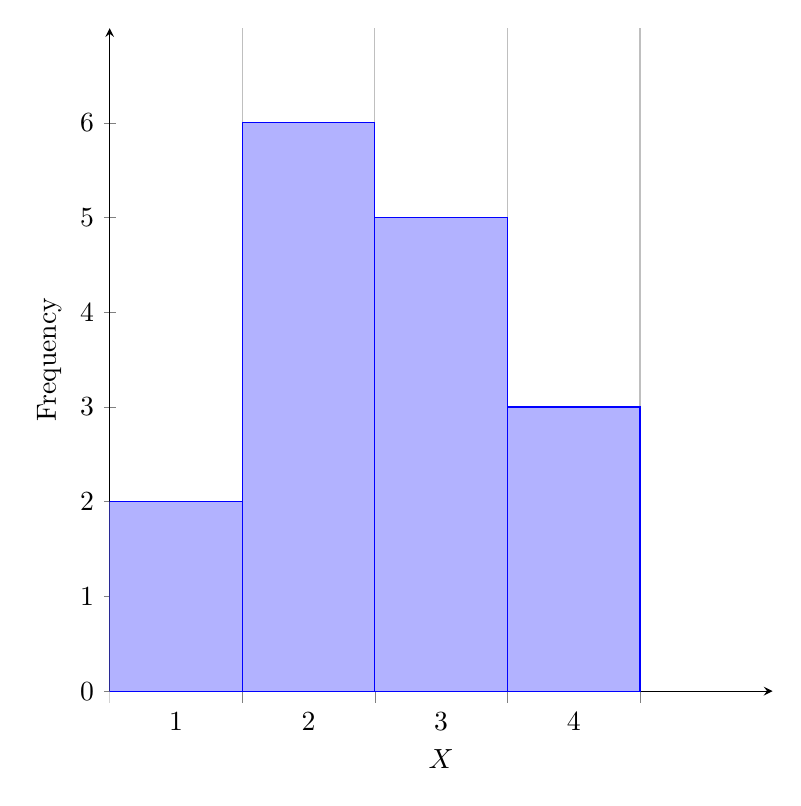
\begin{tikzpicture}
\begin{axis}[
	ylabel=Frequency,xlabel=$X$,
	axis lines=left,
	ymax=7,
	xmax=5,
	ybar interval=1,
	ytick = {0,...,6},
	width=10cm,height=10cm,
]
\addplot
	coordinates {(4,3) (3,5) (2,6) (1,2) (0,0)};
\end{axis}
\end{tikzpicture}
\end{center}
Frequency distributions are good summaries of data because they show the variability in the observed outcomes clearly. Another way to summarize results are single-number summaries such as the following:
\bigskip\par
The \textbf{mean} of a sample of outcomes is the average value of the outcomes. It is the sum of the outcomes divide by the total number of outcomes. The mean of $n$ outcomes, $x_1,\ldots,x_n$, for a random variable $X$ is
\[
    \sum_{i = 0}^{n} \frac{x_i}{n} = \frac{x_1,\ldots,x_n}{n}
\]
\bigskip\par
The \textbf{median} of a sample is an outcome such that half the outcomes are before it and half the outcomes are after it when the outcomes are arranged in numerical order.
\bigskip\par
The \textbf{mode} of a sample is the outcome that occurs most frequently. There can be multiple equal modes in a sample.
\bigskip\par
\begin{example}
A fisherman records the weight of each fish he catches for a week. These are his results. Each value represents the weight, in pounds, of a fish he caught.
\[
    \{\, 20,23,19,27,17,22,18,15,23,25,18,23,29 \,\}
\]
A frequency distribution of the sample above is
\begin{center}
\begin{tabular}{ |c|c|c|c| } 
\hline
$X$ & Frequency Count & Frequency \\
\hline
15 & \StrokeOne & 1 \\ 
17 & \StrokeOne & 1 \\ 
18 & \StrokeTwo & 2 \\ 
19 & \StrokeOne & 1 \\
20 & \StrokeOne & 1 \\
22 & \StrokeOne & 1 \\ 
23 & \StrokeThree & 3 \\ 
25 & \StrokeOne & 1 \\ 
27 & \StrokeOne & 1 \\
29 & \StrokeOne & 1 \\
\hline
\end{tabular}
\end{center}
And the following is a frequency histogram
\begin{center}
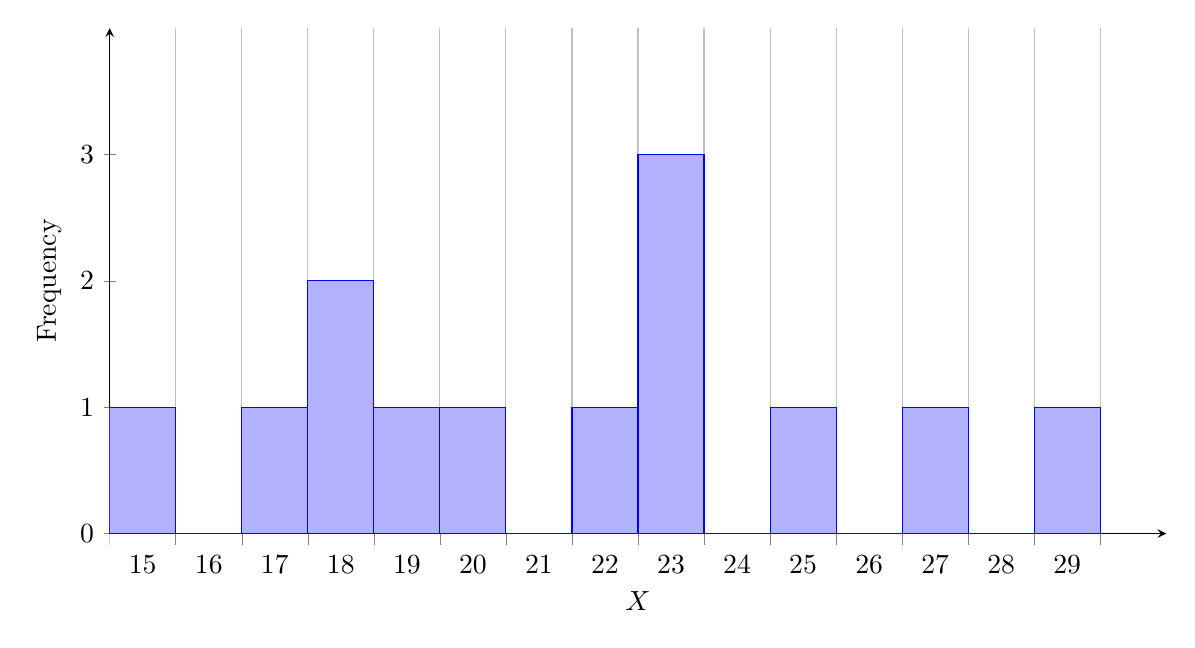
\begin{tikzpicture}
\begin{axis}[
	ylabel=Frequency,xlabel=$X$,
	axis lines=left,
	ymax=4,	
	xmin=14,
	xmax=30,
	ybar interval=1,
	ytick = {0,1,2,3},
	width=15cm,height=8cm,
]
\addplot
	coordinates {(29,1) (28,0) (27,1) (26,0) (25,1) (24,0) (23,3) (22,1) (21,0) (20,1) (19,1) (18,2) (17,1) (16,0) (15,1) (14,0)};
\end{axis}
\end{tikzpicture}
\end{center}
The mean weight of sample of fishes is
\[
    \frac{20+23+19+27+22+18+15+23+18+23+29}{13} = \frac{237}{13} \approx 18.231
\]
The median weight of the sample of fishes is found by rearranging the sample into numerical order and selecting the middle outcome. The median is 22.
\[
    15,18,18,19,20,\underuparrow{22},23,23,23,27,29
\]
The mode is the weight that occurs most frequently. It corresponds to tallest bar on the histogram. 23lbs occurs the most (3 times) so it is the median.
\end{example}

% ------------------------------------------------------ %
\section{Expected Value of a Random Variable}
The expected value of a random variable $X$ with a range of $A$ and a probability function $f(x)$, is given by
\[
    E(X) = \mean = \sum_{x \in A} xf(x)
\]
\begin{info}
Note that in order to calculate the expected value of a random variable $X$, we often need to know the distribution, and hence the probability function, of $X$.
\end{info}
\begin{theory}{Derivation of the Expected Value}
Suppose we have a frequency distribution of a random variable X, as shown below:
\begin{center}
\begin{tabular}{ |c|c|c|c| } 
\hline
$X$ & Frequency Count & Frequency \\
\hline
5 & \StrokeFive\StrokeFive & 10 \\ 
10 & \StrokeFive\StrokeTwo & 7 \\ 
25 & \StrokeFive\StrokeFive\StrokeThree & 13 \\
100 & \StrokeFour & 4 \\
200 & \StrokeTwo & 1 \\ 
\hline
\end{tabular}
\end{center}
As we learnt in the previous section, we can calculate the mean as
\begin{align*}
    &\frac{(5\times10) + (10\times2) + (25\times13) + (100\times4) + (200\times1)}{30} \\
    &= (5)\left(\frac{10}{30}\right) + (10)\left(\frac{7}{30}\right) + (25)\left(\frac{13}{30}\right) + (100)\left(\frac{4}{30}\right) + (200)\left(\frac{1}{30}\right) \\
    \text{($A$ is the range  of $X$) }
    &=\sum_{x \in A} x \times \text{the fraction of times $x$ occurs}
\end{align*}
Now suppose we know the probability function of $X$ is as follows
\renewcommand{\arraystretch}{1.5}
\begin{center}
\begin{tabular}{ c|c c c c c } 
$x$ & 5 & 10 & 25 & 100 & 200 \\
\hline
$f(x)$ & $\frac{1}{3}$ & $\frac{7}{30}$ & $\frac{13}{30}$ & $\frac{2}{15}$ & $\frac{1}{30}$ \\
\end{tabular}
\end{center}
Using the relative frequency definition of probability, we know that if we observed a very large number of outcomes, the fraction of times $X=x$ occurs (relative frequency of $x$) is $f(x)$. \\ Thus, \textit{in theory}, we would expect the mean of a sample of infinitely many outcomes to be
\[
    (5)\left(\frac{1}{3}\right) + (10)\left(\frac{7}{30}\right) + (25)\left(\frac{13}{30}\right) + (100)\left(\frac{2}{15}\right) + (200)\left(\frac{1}{30}\right) \approx 33.167
\]
This theoretical mean is denoted by $\mu$ or $E(X)$, and is known as the expected value of $X$.
\end{theory}
\begin{example}
A slots machine in a casino costs \$5 to play. It has probabilities of 0.5 to pay out \$2, 0.2 to pay out \$5, a 0.1 to pay out \$10 and otherwise does not pay out anything. Let the random variable $X$ be the amount of money (in dollars) the machine pays out in one play, and $Y$ be the amount of money won or lost in one play. Find $E(X)$ and $E(Y)$.
\[
    E(X) = (0)(0.2) + (2)(0.5) + (5)(0.2) + (10)(0.1) = 3
\]
\[
    E(Y) = (-5)(0.2) + (-3)(0.5) + (0)(0.2) + (5)(0.1) = -2
\]
Note that $E(Y) = E(X - 5) = E(X) - 5$
\end{example}

\begin{example}
A nightclub lets groups of up to 6 people enter at reduced fees. A randomly selected group in the nightclub's line has the following probabilities for its size and cost of entry:
\begin{center}
\begin{tabular}{ |c|c|c| } 
\hline
Size of Group (X) & Cost of Entry (Y) & Probability \\
\hline
1 & \$10 & 0.1 \\
2 & \$18 & 0.15 \\
3 & \$26 & 0.1 \\
4 & \$34 & 0.3 \\
5 & \$42 & 0.15 \\
6 & \$50 & 0.2 \\
\hline
\end{tabular}
\end{center}
1. Let $X$ be the size of a randomly selected group. Find $E(X)$.
\[
    E(X) = (0.1)(1) + (0.15)(2) + (0.1)(3) + (0.3)(4) + (0.15)(5) + (0.2)(6) = 3.85
\]
2. If the cost of entry of a group (Y) is $8 \times\text{the size of the group}+2$. Find the expected value of the cost of entry, in dollars, of a randomly selected group.
\[
    E(8X + 2)
    = E(Y) 
    = (0.1)(10) + (0.15)(18) + (0.1)(26) + (0.3)(34) + (0.15)(42) + (0.2)(50)
    = 32.8
\]
3. Show that the expected value of the cost of entry of a randomly selected group is $8 \times \text{the expected value of the size of the group} + 2$.
\[
    8E(X) + 2 = 8 \times 3.85 + 2 = 30.8 + 2 = 32.8 = E(8X + 2)
\]
\end{example}

\begin{theorem}
Let $X$ be a discrete random variable with a range of A, and probability function $f(x)$. The expected value of some function g(X) is given by
\[
    E\left[g(X)\right] = \sum_{x \in A} g(x)f(x)
\]
\end{theorem}
\begin{proof}
Let the random variable $Y = g(X)$ have a range of $B$ and a probability function $f_{\scriptscriptstyle Y}(y) = P(Y = y)$.
\[
    E[g(X)] = E(Y) = \sum_{y \in B} yf_{\scriptscriptstyle Y}(y)
\]
Now, let $C_y$ be $\{\, x \ssep g(x) = y \,\}$, that is the set of all values of $x$ such that $g(X)$ is $y$. So
\[
    f_{\scriptscriptstyle Y}(y) = P[g(X) = y]=\sum_{x \in C_y} f(x)
\]
That is, the probability that $Y = y$ is the sum of the probabilities that $X = x$ such that $g(x) = y$. \\
Now, we have
\begin{align*}
    E[g(X)] &= \sum_{y \in B} yf_{\scriptscriptstyle Y}(y) 
             = \sum_{y \in B} y\sum_{x \in C_y}  f(x) 
             = \sum_{y \in B}  \sum_{x \in C_y} yf(x) \\
            &= \sum_{y \in B}  \sum_{x \in C_y}  g(x)f(x)&
\end{align*}
Note that the inner summation is for all $x$ such that $g(x) = y$ and the outer is for all $y$. Thus the equation is the sum for all $x$. So
\[
    E[g(X)] = \sum_{y \in B} \sum_{x \in C_y} g(x)f(x) 
            = \sum_{x \in A} g(x)f(x)
\]
where $A$ is the range of X, as required.
\end{proof}

\subsection*{Linear Properties of Expected Value}
\begin{theorem}
For constants $a,b$ and $c$,
\[
    E[ag_1(X) + bg_2(X) + c] = aE[g_1(X)] + bE[g_2(X)] + c
\]
\end{theorem}
\begin{proof}
\begin{align*}
    E[aE[g_1(X)] + bE[g_2(X)]+c]
    &= \sum_{\all x} [ag_1(x)+bg_2(x)+c]f(x) \\
    &= \sum_{\all x} [ag_1(x)f(x)+bg_2(x)f(x)+cf(x)] \\
    &= \sum_{\all x}ag_1(x)f(x)+\sum_{\all x}bg_2(x)f(x)+\sum_{\all x}cf(x) \\
    &= a\sum_{\all x}g_1(x)f(x)+b\sum_{\all x}g_2(x)f(x)+c\sum_{\all x}f(x) \\
    \left(\text{recall }\sum_{\all x}f(x) = 1\right) \hspace{1cm}
    &= aE[g_1(X)] + b[g_2(X)] + c
\end{align*}
\end{proof}
% ====================================================== %

\section{Variance of a Random Variable}
The variance of a random variable~$X$ is given by
\[
    \var(X) = \stddev^2 = E\left[(X - \mean)^2\right]
\]
where $\stddev$ is the standard deviation of $X$. It is the average squared deviation of a random variable from its mean. It measures how far out from the mean the values of a random variable are spread.
\smallskip\par
The definition and formula above is useful in understanding the variance's importance but it can be difficult to use to actually calculate the variance. Here are a few other useful formulas for calculating the variance of a random variable:
\begin{align}
    \var(X) &= E(X^2) - [E(X)]^2 = E(X^2) - \mean^2 \label{eqn: variance alt formula}\\
    \var(X) &= E[X(X-1)] + E(X) - [E(X)]^2 = E[X(X-1)] + \mean - \mean^2
\end{align}
\begin{theory}{Derivation of Alternative Formulas}
\begin{align*}
    \var(X) = \stddev^2 
    &= E\left[(X - \mean)^2\right] \\
    &= E\left[X^2 -2X\mean + \mean^2\right] \\
    &= E(X^2) - 2\mean E(X) + \mean^2,\:\text{(by linear property since $\mean$ is a constant)} \\
    &= E(X^2) - 2\mean^2 + \mean^2,\:\text{(since $E(X) = \mean$)} \\
    &= E(X^2) - \mean^2
\end{align*}
Now note that $X^2 = X(X-1) + X$, so we have
\begin{align*}
    \var(X) = \stddev^2
    &= E[X(X-1) + X]  - \mean^2 \\
    &= E[X(X-1)] + E(X) -\mean^2 \\
    &= E[X(X-1)] + \mean -\mean^2
\end{align*}
\end{theory}
\subsection*{Properties of Variance}
\begin{theorem}
For constants $a$ and~$b$,
\[
    \var[aX + b] = a^2\var(X)
\]
\end{theorem}
\begin{proof}
\begin{align*}
    \var[aX + b]
    &= E\bigl[(aX + b)^2\bigr] - \bigl[E(aX + b)\bigr]^2,\hspace{12pt}\text{\big (by equation \eqref{eqn: variance alt formula}\big)} \\
    &= E\bigl[a^2 X^2 + 2abX + b^2\bigr] - \bigl[aE(X) + b\bigr]^2 \\
    &= a^2 E(X^2) + 2ab E(X) + b^2 - a^2[E(X)]^2 - 2abE(X) - b^2 \\
    &= a^2 \left(E(X^2) - [E(X)]^2\right) \\
    &= a^2 \var(X)
\end{align*}
\end{proof}
\subsection{Standard Deviation of a Random Variable}
The standard deviation of a random variable~$X$ is defined as
\[
    \stddev = \sqrt{\mathstrut\var X} 
    = \sqrt{\mathstrut E\bigl[(X - \mean)^2\bigr]}
\]
It is another measure used to quantify the variability of a random variable.
\begin{info}
A useful property of the standard deviation is that it is expressed in the same units as the random variable, unlike the variance.
\end{info}
\end{document}
